% Week 8: Natural Language Processing II - Attention and Transformers
\chapter{Week 8: NLP II - Attention and Transformers}
\label{ch:week8}

\begin{quickref}[Chapter Overview]
\textbf{Core goal:} Understand the attention mechanism and transformer architecture that revolutionised modern deep learning.

\textbf{Key topics:}
\begin{itemize}
    \item Encoder-decoder architecture for sequence-to-sequence tasks
    \item Machine translation and the BLEU evaluation metric
    \item Attention mechanism: biological inspiration, queries, keys, and values
    \item Scoring functions: additive and scaled dot-product attention
    \item Bahdanau attention, multi-head attention, and self-attention
    \item Positional encoding for sequence order
    \item Transformer architecture (encoder-only, decoder-only, encoder-decoder)
    \item Pretrained models: BERT and Vision Transformer (ViT)
\end{itemize}

\textbf{Key equations:}
\begin{itemize}
    \item Scaled dot-product attention: $a(\mathbf{q}, \mathbf{k}) = \text{softmax}\left(\frac{\mathbf{q}^\top \mathbf{k}}{\sqrt{d}}\right)$
    \item Self-attention output: $\mathbf{y}_i = \sum_{j=1}^{n} \alpha(\mathbf{x}_i, \mathbf{x}_j) \mathbf{x}_j$
    \item Bahdanau context: $\mathbf{c}_{t'} = \sum_{t=1}^{T} \alpha(\mathbf{s}_{t'-1}, \mathbf{h}_t) \mathbf{h}_t$
\end{itemize}
\end{quickref}

%==============================================================================
\section{Encoder-Decoder Architecture}
\label{sec:encoder-decoder}
%==============================================================================

The encoder-decoder architecture is the foundational framework for sequence-to-sequence (seq2seq) problems, where we must transform an input sequence into an output sequence of potentially different length. This architecture underpins machine translation, text summarisation, dialogue systems, and question answering.

\subsection{Machine Translation: A Motivating Example}

Machine translation is the canonical seq2seq problem. Given a sentence in a \textbf{source language} (e.g., English), the model must produce the corresponding sentence in a \textbf{target language} (e.g., German).

\begin{rigour}[Machine Translation Problem]
\textbf{Definition:} Machine translation maps an input sequence $\mathbf{x} = (x_1, x_2, \ldots, x_T)$ in the source language to an output sequence $\mathbf{y} = (y_1, y_2, \ldots, y_{T'})$ in the target language.

\textbf{Key challenges:}
\begin{itemize}
    \item \textbf{Variable lengths:} Source and target sentences may have different numbers of tokens ($T \neq T'$)
    \item \textbf{Non-monotonic alignment:} Corresponding words may appear in different positions across languages
\end{itemize}

\textbf{Example:}
\begin{align*}
    \text{English:} & \quad \text{``I would like to learn German.''} \\
    \text{German:} & \quad \text{``Ich m\"{o}chte Deutsch lernen.''}
\end{align*}

The word ``German'' (position 6 in English) corresponds to ``Deutsch'' (position 3 in German), demonstrating the non-monotonic alignment challenge.
\end{rigour}

\begin{figure}[H]
    \centering
    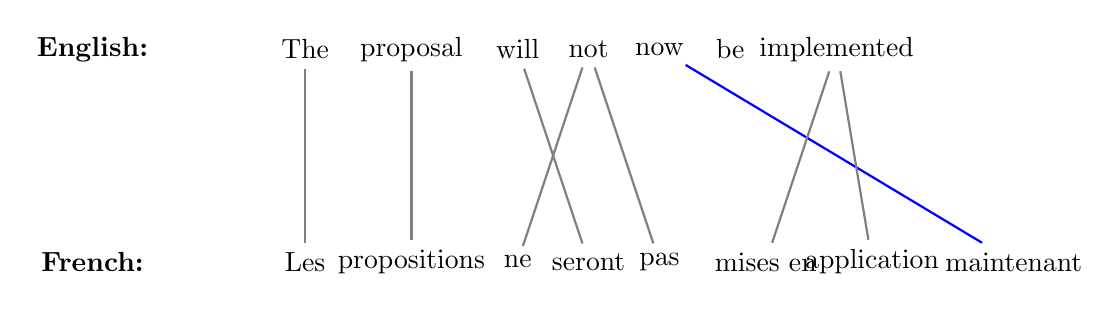
\begin{tikzpicture}[scale=0.9]
        % English sentence
        \node at (-3, 2) {\textbf{English:}};
        \node (e1) at (0, 2) {The};
        \node (e2) at (1.5, 2) {proposal};
        \node (e3) at (3, 2) {will};
        \node (e4) at (4, 2) {not};
        \node (e5) at (5, 2) {now};
        \node (e6) at (6, 2) {be};
        \node (e7) at (7.5, 2) {implemented};

        % French sentence
        \node at (-3, -1) {\textbf{French:}};
        \node (f1) at (0, -1) {Les};
        \node (f2) at (1.5, -1) {propositions};
        \node (f3) at (3, -1) {ne};
        \node (f4) at (4, -1) {seront};
        \node (f5) at (5, -1) {pas};
        \node (f6) at (6.5, -1) {mises en};
        \node (f7) at (8, -1) {application};
        \node (f8) at (10, -1) {maintenant};

        % Alignment lines (showing non-monotonic alignment)
        \draw[-, gray, thick] (e1) -- (f1);
        \draw[-, gray, thick] (e2) -- (f2);
        \draw[-, gray, thick] (e3) -- (f4);
        \draw[-, gray, thick] (e4) -- (f3);
        \draw[-, gray, thick] (e4) -- (f5);
        \draw[-, blue, thick] (e5) -- (f8);  % Crossing alignment
        \draw[-, gray, thick] (e7) -- (f6);
        \draw[-, gray, thick] (e7) -- (f7);
    \end{tikzpicture}
    \caption{Word alignment between English and French (adapted from Brown et al., 1990). Note the crossing alignments: ``now'' at position 5 in English maps to ``maintenant'' at position 9 in French, while ``implemented'' maps to a multi-word phrase. These non-monotonic alignments are a key challenge in machine translation.}
    \label{fig:word-alignment}
\end{figure}

\begin{quickref}[Other Seq2Seq Applications]
Beyond machine translation, the encoder-decoder framework applies to:
\begin{itemize}
    \item \textbf{Question answering:} Input question $\rightarrow$ output answer
    \item \textbf{Dialogue systems:} User utterance $\rightarrow$ system response
    \item \textbf{Text summarisation:} Long document $\rightarrow$ concise summary
    \item \textbf{Code generation:} Natural language description $\rightarrow$ code
\end{itemize}
\end{quickref}

\subsection{The Encoder-Decoder Framework}

The encoder-decoder architecture addresses variable-length sequence transformation by introducing an intermediate fixed-dimensional representation.

\begin{rigour}[Encoder-Decoder Architecture]
The architecture consists of two components:

\textbf{1. Encoder:} Takes a variable-length input sequence and transforms it into a \textbf{fixed-shape state} (context):
\[
\text{Encoder}: (x_1, x_2, \ldots, x_T) \longrightarrow \mathbf{c} \in \mathbb{R}^h
\]

\textbf{2. Decoder:} Takes the fixed-shape context and generates a variable-length output sequence:
\[
\text{Decoder}: \mathbf{c} \longrightarrow (y_1, y_2, \ldots, y_{T'})
\]

\textbf{Information flow:}
\[
\text{Input sequence} \xrightarrow{\text{Encoder}} \text{Context } \mathbf{c} \xrightarrow{\text{Decoder}} \text{Output sequence}
\]

The context vector $\mathbf{c}$ acts as an information bottleneck, compressing the entire input sequence into a fixed-dimensional representation that the decoder must use to generate the output.
\end{rigour}

\begin{figure}[H]
    \centering
    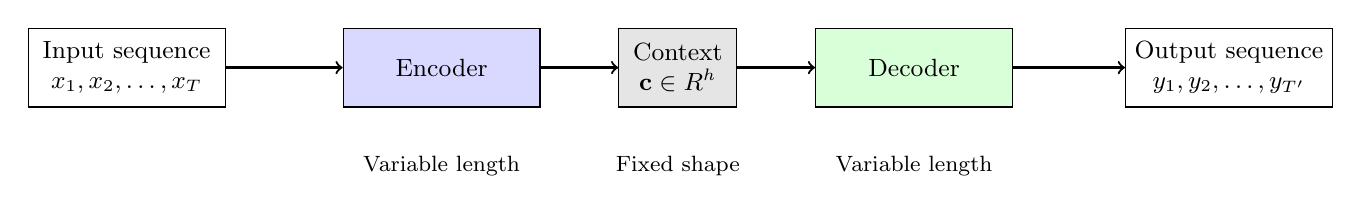
\begin{tikzpicture}[
        box/.style={rectangle, draw, minimum width=2.5cm, minimum height=1cm, align=center, font=\small},
        state/.style={rectangle, draw, fill=gray!20, minimum width=1.5cm, minimum height=1cm, align=center, font=\small},
        arrow/.style={->, thick}
    ]
        \node[box] (input) at (0, 0) {Input sequence\\$x_1, x_2, \ldots, x_T$};
        \node[box, fill=blue!15] (encoder) at (4, 0) {Encoder};
        \node[state] (context) at (7, 0) {Context\\$\mathbf{c} \in \mathbb{R}^h$};
        \node[box, fill=green!15] (decoder) at (10, 0) {Decoder};
        \node[box] (output) at (14, 0) {Output sequence\\$y_1, y_2, \ldots, y_{T'}$};

        \draw[arrow] (input) -- (encoder);
        \draw[arrow] (encoder) -- (context);
        \draw[arrow] (context) -- (decoder);
        \draw[arrow] (decoder) -- (output);

        \node[below=0.3cm] at (4, -0.7) {\footnotesize Variable length};
        \node[below=0.3cm] at (7, -0.7) {\footnotesize Fixed shape};
        \node[below=0.3cm] at (10, -0.7) {\footnotesize Variable length};
    \end{tikzpicture}
    \caption{Encoder-decoder architecture: the encoder compresses a variable-length input into a fixed-dimensional context vector, which the decoder expands into a variable-length output.}
    \label{fig:encoder-decoder-flow}
\end{figure}

\subsection{Autoencoder: A Special Case}

When the source and target domains are identical, the encoder-decoder becomes an \textbf{autoencoder}-a model that learns to reconstruct its input.

\begin{rigour}[Autoencoder]
\textbf{Definition:} An autoencoder is an encoder-decoder where the target output equals the input:
\[
\text{Autoencoder}: \mathbf{x} \xrightarrow{\text{Encoder}} \mathbf{z} \xrightarrow{\text{Decoder}} \hat{\mathbf{x}} \approx \mathbf{x}
\]

The intermediate representation $\mathbf{z}$ (called the \textbf{latent code}) typically has lower dimensionality than $\mathbf{x}$, forcing the model to learn a compressed representation.

\textbf{Training objective:} Minimise reconstruction error, e.g., $\|\mathbf{x} - \hat{\mathbf{x}}\|^2$.

\textbf{Variants:}
\begin{itemize}
    \item \textbf{Regularised autoencoders:} Add constraints on $\mathbf{z}$ for downstream classification
    \item \textbf{Variational autoencoders (VAEs):} Impose probabilistic structure on $\mathbf{z}$ for generative modelling
    \item \textbf{Denoising autoencoders:} Reconstruct clean input from corrupted input
\end{itemize}

\textbf{Applications:}
\begin{itemize}
    \item Dimensionality reduction (alternative to PCA)
    \item Anomaly detection (high reconstruction error indicates anomaly)
    \item Image compression and denoising
    \item Learning representations for downstream tasks
\end{itemize}
\end{rigour}

\subsection{RNN-Based Encoder-Decoder}

The vanilla implementation uses recurrent neural networks for both encoder and decoder components.

\begin{rigour}[RNN Encoder]
Given an input sequence of tokens $x_1, x_2, \ldots, x_T$, the encoder RNN processes each token sequentially:
\[
\mathbf{h}_t = f(\mathbf{x}_t, \mathbf{h}_{t-1})
\]
where:
\begin{itemize}
    \item $\mathbf{h}_t \in \mathbb{R}^h$ is the hidden state at time $t$
    \item $\mathbf{x}_t$ is the embedding of token $x_t$
    \item $f$ is the recurrent function (e.g., LSTM, GRU cell)
    \item $\mathbf{h}_0$ is typically initialised to zeros
\end{itemize}

The encoder transforms the hidden states into a \textbf{context variable} via a function $q$:
\[
\mathbf{c} = q(\mathbf{h}_1, \mathbf{h}_2, \ldots, \mathbf{h}_T)
\]

\textbf{Simple choice:} Use only the final hidden state: $\mathbf{c} = \mathbf{h}_T$.

This is computationally simple but problematic for long sequences, as early tokens must survive many recurrent steps to influence the context.
\end{rigour}

\begin{rigour}[RNN Decoder]
Given the context $\mathbf{c}$ and target sequence $y_1, y_2, \ldots, y_{T'}$, the decoder generates output tokens autoregressively.

At each time step $t'$, the decoder:
\begin{enumerate}
    \item Computes a hidden state using the previous token and context:
    \[
    \mathbf{s}_{t'} = g(y_{t'-1}, \mathbf{c}, \mathbf{s}_{t'-1})
    \]
    \item Predicts a probability distribution over the vocabulary:
    \[
    P(y_{t'+1} \mid y_1, \ldots, y_{t'}, \mathbf{c})
    \]
\end{enumerate}

\textbf{Implementation details:}
\begin{itemize}
    \item The encoder's final hidden state $\mathbf{h}_T$ initialises the decoder's hidden state $\mathbf{s}_0$
    \item The context $\mathbf{c}$ is concatenated with decoder input at \textit{every} time step
    \item A fully connected layer transforms the decoder hidden state to vocabulary-sized logits
    \item Softmax produces the probability distribution over next tokens
\end{itemize}
\end{rigour}

\begin{redbox}
\textbf{Training vs Inference Discrepancy (Teacher Forcing)}

\textbf{During training:}
\begin{itemize}
    \item The \textbf{ground truth} token $y_{t'}$ is fed as input at time $t'+1$
    \item This is called \textbf{teacher forcing}-the model is ``told'' the correct previous token
    \item Enables efficient parallel training with known targets
\end{itemize}

\textbf{During inference:}
\begin{itemize}
    \item The \textbf{predicted} token $\hat{y}_{t'}$ is fed as input at time $t'+1$
    \item Errors can compound: a wrong prediction leads to increasingly wrong context
    \item The model never saw its own mistakes during training
\end{itemize}

This train-test mismatch is called \textbf{exposure bias} and can degrade inference quality, particularly for long sequences.
\end{redbox}

\subsection{Data Preprocessing for Machine Translation}

\begin{quickref}[Preprocessing Steps]
\textbf{Data sources:} Parallel corpora such as the Tatoeba Project provide aligned sentence pairs across many languages.

\textbf{Tokenisation:} Typically word-level tokenisation, though subword methods (BPE, WordPiece) are now standard.

\textbf{Minibatch handling:} Since sentences have variable lengths, batching requires:
\begin{enumerate}
    \item \textbf{Truncation:} Keep only the first $L$ tokens; discard the rest
    \item \textbf{Padding:} Append special \texttt{<pad>} tokens to reach length $L$
\end{enumerate}

Special tokens:
\begin{itemize}
    \item \texttt{<pad>}: Padding for batch alignment
    \item \texttt{<bos>}: Beginning of sequence (decoder start)
    \item \texttt{<eos>}: End of sequence (signals completion)
    \item \texttt{<unk>}: Unknown/out-of-vocabulary tokens
\end{itemize}
\end{quickref}

%==============================================================================
\section{BLEU: Evaluating Machine Translation}
\label{sec:bleu}
%==============================================================================

Evaluating translation quality is challenging because multiple valid translations exist for any source sentence. The BLEU metric provides an automatic evaluation method.

\begin{rigour}[BLEU Score]
\textbf{BLEU (Bilingual Evaluation Understudy)} compares predicted sequences against reference translations using n-gram precision.

\textbf{N-gram precision $p_n$:} The ratio of matched n-grams to total n-grams in the prediction:
\[
p_n = \frac{\text{Number of n-grams in prediction matching reference}}{\text{Total n-grams in prediction}}
\]

\textbf{BLEU formula:}
\[
\text{BLEU} = \exp\left(\min\left(0, 1 - \frac{\text{len}_{\text{label}}}{\text{len}_{\text{pred}}}\right)\right) \prod_{n=1}^{k} p_n^{1/2^n}
\]

where:
\begin{itemize}
    \item $\text{len}_{\text{label}}$ = number of tokens in reference (target) sequence
    \item $\text{len}_{\text{pred}}$ = number of tokens in predicted sequence
    \item $k$ = maximum n-gram length to consider (typically 4)
    \item $p_n$ = precision of n-grams of length $n$
\end{itemize}

\textbf{Components explained:}
\begin{enumerate}
    \item \textbf{Brevity penalty:} The exponential term penalises predictions shorter than the reference. If $\text{len}_{\text{pred}} \geq \text{len}_{\text{label}}$, the penalty is 1.
    \item \textbf{Weighted geometric mean:} The product $\prod_{n=1}^{k} p_n^{1/2^n}$ combines precisions, with exponentially decreasing weights ($1/2, 1/4, 1/8, \ldots$) for longer n-grams.
\end{enumerate}
\end{rigour}

\begin{quickref}[BLEU Properties]
\textbf{Perfect score:} BLEU = 1 when prediction exactly matches reference.

\textbf{Higher n-gram weighting:} Longer n-grams receive higher weights because they are harder to match by chance. Matching a 4-gram is much more indicative of quality than matching individual words.

\textbf{Limitations:}
\begin{itemize}
    \item Does not account for synonyms or paraphrases
    \item Insensitive to word order beyond n-gram level
    \item May not correlate well with human judgement for short texts
\end{itemize}

\textbf{Practical use:} BLEU is widely used for comparing systems and tracking progress, but should be complemented by human evaluation for final assessment.
\end{quickref}

\begin{rigour}[BLEU Worked Example]
Consider:
\begin{itemize}
    \item Reference: ``the cat sat on the mat'' (6 tokens)
    \item Prediction: ``the cat on the mat'' (5 tokens)
\end{itemize}

\textbf{Unigram precision ($p_1$):}
\begin{itemize}
    \item Prediction unigrams: \{the, cat, on, the, mat\} (5 tokens)
    \item Matches in reference: all 5 match
    \item $p_1 = 5/5 = 1.0$
\end{itemize}

\textbf{Bigram precision ($p_2$):}
\begin{itemize}
    \item Prediction bigrams: \{the-cat, cat-on, on-the, the-mat\} (4 bigrams)
    \item Reference bigrams: \{the-cat, cat-sat, sat-on, on-the, the-mat\}
    \item Matches: the-cat, on-the, the-mat (3 matches)
    \item $p_2 = 3/4 = 0.75$
\end{itemize}

\textbf{Brevity penalty:}
\[
\text{BP} = \exp\left(\min\left(0, 1 - \frac{6}{5}\right)\right) = \exp(-0.2) \approx 0.819
\]

\textbf{BLEU (using $k=2$):}
\[
\text{BLEU} = 0.819 \times (1.0)^{0.5} \times (0.75)^{0.25} \approx 0.819 \times 1.0 \times 0.930 \approx 0.76
\]
\end{rigour}

%==============================================================================
\section{The Attention Mechanism}
\label{sec:attention}
%==============================================================================

The attention mechanism addresses a fundamental limitation of vanilla encoder-decoder models and has become the cornerstone of modern deep learning.

\subsection{The Problem: Information Bottleneck}

\begin{redbox}
\textbf{The Long Sequence Problem}

In vanilla RNN encoder-decoder models:
\begin{itemize}
    \item Only the \textbf{final hidden state} $\mathbf{h}_T$ is passed to the decoder
    \item The entire input sequence must be compressed into a single fixed-dimensional vector
    \item For long sequences, information from early tokens is progressively ``forgotten''
    \item The decoder uses the \textbf{same context} $\mathbf{c}$ regardless of which output token it is generating
\end{itemize}

This is problematic because not all input tokens are equally relevant to each output token. When translating ``I would like to learn German'', the context needed for ``lernen'' (learn) differs from that needed for ``Deutsch'' (German).
\end{redbox}

\subsection{Biological Inspiration}

The attention mechanism draws inspiration from human visual and cognitive attention.

\begin{quickref}[Attention in Biology]
\textbf{The problem:} Our optical nerve receives far more sensory input than the brain can fully process.

\textbf{The solution:} We selectively focus on objects of interest, freeing cognitive capacity.

\textbf{Key properties of biological attention:}
\begin{itemize}
    \item \textbf{Selective focus:} We concentrate on a small fraction of available information
    \item \textbf{Cognitive control:} Attention can be directed volitionally (goal-directed)
    \item \textbf{Automatic capture:} Salient stimuli can capture attention involuntarily
    \item \textbf{Resource scarcity:} Attention has opportunity cost-focusing on one thing means ignoring others
\end{itemize}

The deep learning attention mechanism mirrors this: instead of using all information equally, the model learns to focus on relevant parts of the input for each output decision.
\end{quickref}

\subsection{Attention Cues: Volitional and Non-Volitional}

\begin{rigour}[Types of Attention Cues]
\textbf{1. Non-volitional cues (bottom-up):}
\begin{itemize}
    \item Based on \textbf{saliency and conspicuity} of objects
    \item Automatic, stimulus-driven
    \item Example: A bright red object in a grey scene captures attention
\end{itemize}

\textbf{2. Volitional cues (top-down):}
\begin{itemize}
    \item Based on \textbf{variable selection criteria}
    \item Deliberate, goal-directed
    \item Example: Searching for a specific word on a page
\end{itemize}

In neural attention:
\begin{itemize}
    \item Non-volitional $\approx$ content-based similarity (what is salient in the input)
    \item Volitional $\approx$ query-based retrieval (what we are looking for)
\end{itemize}
\end{rigour}

\subsection{Queries, Keys, and Values}

The attention mechanism formalises selective focus using three components.

\begin{rigour}[Query-Key-Value Framework]
\textbf{Terminology:}
\begin{itemize}
    \item \textbf{Query} ($\mathbf{q}$): What we are looking for (volitional cue)
    \item \textbf{Keys} ($\mathbf{k}_1, \ldots, \mathbf{k}_n$): Identifiers for each piece of available information (non-volitional cues)
    \item \textbf{Values} ($\mathbf{v}_1, \ldots, \mathbf{v}_n$): The actual information content
\end{itemize}

\textbf{Structure:} Each value is paired with a key: $\{(\mathbf{k}_1, \mathbf{v}_1), \ldots, (\mathbf{k}_n, \mathbf{v}_n)\}$.

\textbf{Attention mechanism:}
\begin{enumerate}
    \item Compare query to all keys to compute \textbf{attention scores}
    \item Convert scores to \textbf{attention weights} (typically via softmax)
    \item Compute weighted sum of values as the \textbf{attention output}
\end{enumerate}

\textbf{Intuition:} The query ``asks a question''; keys determine relevance; values provide the answer. High query-key similarity means the corresponding value contributes more to the output.
\end{rigour}

\begin{figure}[H]
    \centering
    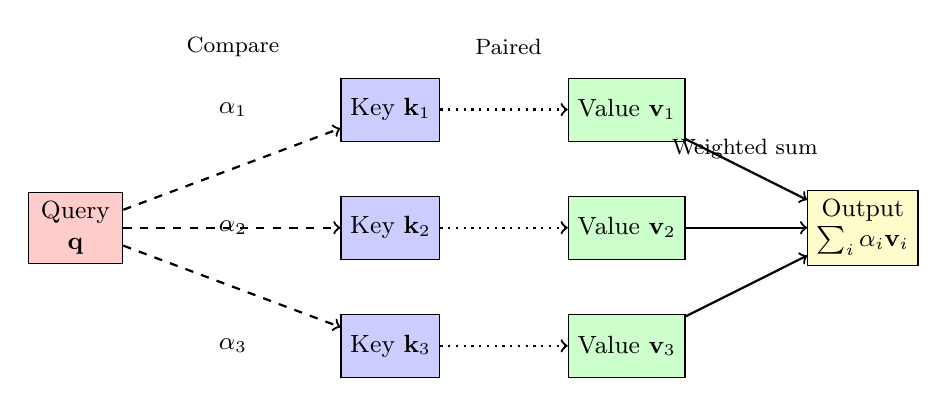
\begin{tikzpicture}[
        query/.style={rectangle, draw, fill=red!20, minimum width=1.2cm, minimum height=0.8cm, align=center, font=\small},
        key/.style={rectangle, draw, fill=blue!20, minimum width=1.2cm, minimum height=0.8cm, align=center, font=\small},
        value/.style={rectangle, draw, fill=green!20, minimum width=1.2cm, minimum height=0.8cm, align=center, font=\small},
        output/.style={rectangle, draw, fill=yellow!20, minimum width=1.2cm, minimum height=0.8cm, align=center, font=\small},
        arrow/.style={->, thick}
    ]
        % Query
        \node[query] (q) at (0, 0) {Query\\$\mathbf{q}$};

        % Keys and Values
        \node[key] (k1) at (4, 1.5) {Key $\mathbf{k}_1$};
        \node[key] (k2) at (4, 0) {Key $\mathbf{k}_2$};
        \node[key] (k3) at (4, -1.5) {Key $\mathbf{k}_3$};

        \node[value] (v1) at (7, 1.5) {Value $\mathbf{v}_1$};
        \node[value] (v2) at (7, 0) {Value $\mathbf{v}_2$};
        \node[value] (v3) at (7, -1.5) {Value $\mathbf{v}_3$};

        % Scores
        \node at (2, 1.5) {\small $\alpha_1$};
        \node at (2, 0) {\small $\alpha_2$};
        \node at (2, -1.5) {\small $\alpha_3$};

        % Output
        \node[output] (out) at (10, 0) {Output\\$\sum_i \alpha_i \mathbf{v}_i$};

        % Arrows from query to keys
        \draw[arrow, dashed] (q) -- (k1);
        \draw[arrow, dashed] (q) -- (k2);
        \draw[arrow, dashed] (q) -- (k3);

        % Arrows from keys to values (pairing)
        \draw[arrow, dotted] (k1) -- (v1);
        \draw[arrow, dotted] (k2) -- (v2);
        \draw[arrow, dotted] (k3) -- (v3);

        % Arrows from values to output
        \draw[arrow] (v1) -- (out);
        \draw[arrow] (v2) -- (out);
        \draw[arrow] (v3) -- (out);

        % Labels
        \node at (2, 2.3) {\footnotesize Compare};
        \node at (5.5, 2.3) {\footnotesize Paired};
        \node at (8.5, 1) {\footnotesize Weighted sum};
    \end{tikzpicture}
    \caption{The query-key-value attention mechanism. The query is compared to all keys to produce attention weights $\alpha_i$. Each key is paired with a value, and the output is a weighted sum of values.}
    \label{fig:qkv-attention}
\end{figure}

\subsection{Attention Pooling}

\begin{rigour}[Attention Pooling]
\textbf{General form:} Given query $\mathbf{q}$ and key-value pairs $\{(\mathbf{k}_i, \mathbf{v}_i)\}_{i=1}^n$, the attention output is:
\[
\text{Attention}(\mathbf{q}, \{(\mathbf{k}_i, \mathbf{v}_i)\}) = \sum_{i=1}^{n} \alpha(\mathbf{q}, \mathbf{k}_i) \mathbf{v}_i
\]
where $\alpha(\mathbf{q}, \mathbf{k}_i)$ is the attention weight for key $\mathbf{k}_i$.

\textbf{Non-parametric example: Nadaraya-Watson kernel regression}
\[
f(x) = \sum_{i=1}^{n} \frac{K(x - x_i)}{\sum_{j=1}^{n} K(x - x_j)} y_i = \sum_{i=1}^{n} \alpha(x, x_i) y_i
\]
where:
\begin{itemize}
    \item $x$ is the query
    \item $(x_i, y_i)$ are key-value pairs
    \item $K(\cdot)$ is a kernel function (e.g., Gaussian)
    \item $\alpha(x, x_i)$ is the normalised attention weight
\end{itemize}

This is \textbf{non-parametric}: the form of attention is fixed by the kernel choice.

\textbf{Parametric attention pooling:} Introduce learnable parameters into the attention computation. With a Gaussian kernel and learnable width $w$:
\[
f(x) = \sum_{i=1}^{n} \text{softmax}\left(-\frac{1}{2}[(x - x_i)w]^2\right) y_i
\]
The parameter $w$ is learned from data, allowing the model to adapt the attention pattern.
\end{rigour}

\subsection{Attention Scoring Functions}

The scoring function determines how query-key similarity is computed before normalisation.

\begin{rigour}[Additive Attention]
\textbf{Use case:} When queries and keys have \textbf{different dimensions}: $\mathbf{q} \in \mathbb{R}^{d_q}$, $\mathbf{k} \in \mathbb{R}^{d_k}$.

\textbf{Scoring function:}
\[
a(\mathbf{q}, \mathbf{k}) = \mathbf{w}_v^\top \tanh(\mathbf{W}_q \mathbf{q} + \mathbf{W}_k \mathbf{k}) \in \mathbb{R}
\]

\textbf{Parameters:}
\begin{itemize}
    \item $\mathbf{W}_q \in \mathbb{R}^{h \times d_q}$: Projects query to hidden dimension $h$
    \item $\mathbf{W}_k \in \mathbb{R}^{h \times d_k}$: Projects key to hidden dimension $h$
    \item $\mathbf{w}_v \in \mathbb{R}^h$: Maps combined representation to scalar score
\end{itemize}

\textbf{Computation:}
\begin{enumerate}
    \item Project query and key to common dimension $h$
    \item Add projections and apply $\tanh$ non-linearity
    \item Linear projection to scalar score
\end{enumerate}

\textbf{Complexity:} $O(h \cdot (d_q + d_k))$ per query-key pair.
\end{rigour}

\begin{rigour}[Scaled Dot-Product Attention]
\textbf{Use case:} When queries and keys have the \textbf{same dimension}: $\mathbf{q}, \mathbf{k} \in \mathbb{R}^d$.

\textbf{Scoring function:}
\[
a(\mathbf{q}, \mathbf{k}) = \frac{\mathbf{q}^\top \mathbf{k}}{\sqrt{d}}
\]

\textbf{Full attention computation:}
\[
\text{Attention}(\mathbf{q}, \mathbf{K}, \mathbf{V}) = \text{softmax}\left(\frac{\mathbf{q}^\top \mathbf{K}}{\sqrt{d}}\right) \mathbf{V}
\]

where $\mathbf{K}$ and $\mathbf{V}$ are matrices with keys and values as rows.

\textbf{Why scale by $\sqrt{d}$?}

For large $d$, the dot product $\mathbf{q}^\top \mathbf{k}$ can have large magnitude. If $q_i, k_i \sim \mathcal{N}(0, 1)$ independently:
\[
\mathbb{E}[\mathbf{q}^\top \mathbf{k}] = 0, \quad \text{Var}(\mathbf{q}^\top \mathbf{k}) = d
\]

Large variance pushes softmax into regions with tiny gradients. Scaling by $\sqrt{d}$ normalises variance to 1.
\end{rigour}

\begin{quickref}[Scaled Dot-Product Attention: Key Properties]
\textbf{Advantages over additive attention:}
\begin{itemize}
    \item \textbf{No learnable parameters} in the scoring function itself
    \item \textbf{Highly parallelisable:} Matrix multiplication is efficiently implemented on GPUs
    \item \textbf{Computationally efficient:} $O(d)$ per query-key pair vs $O(h \cdot 2d)$ for additive
\end{itemize}

\textbf{This is the attention mechanism used in Transformers.}
\end{quickref}

%==============================================================================
\section{Bahdanau Attention}
\label{sec:bahdanau}
%==============================================================================

Bahdanau attention (2015) was the first major application of attention to machine translation, allowing the decoder to focus on different parts of the input for each output token.

\begin{rigour}[Bahdanau Attention]
\textbf{Problem with vanilla encoder-decoder:}
The same context vector $\mathbf{c}$ is used at every decoding step, regardless of which output token is being generated.

\textbf{Solution:} Compute a \textbf{different context vector} $\mathbf{c}_{t'}$ for each decoder time step $t'$:
\[
\mathbf{c}_{t'} = \sum_{t=1}^{T} \alpha(\mathbf{s}_{t'-1}, \mathbf{h}_t) \mathbf{h}_t
\]

\textbf{Components:}
\begin{itemize}
    \item \textbf{Query:} Previous decoder hidden state $\mathbf{s}_{t'-1}$
    \item \textbf{Keys and Values:} Encoder hidden states $\mathbf{h}_1, \ldots, \mathbf{h}_T$ (same for both)
    \item \textbf{Attention weights:} $\alpha(\mathbf{s}_{t'-1}, \mathbf{h}_t)$ computed via additive attention
\end{itemize}

\textbf{Intuition:} When generating output token $y_{t'}$, the model can ``look back'' at the input and focus on the most relevant source tokens. The attention weights $\alpha$ form a soft alignment between source and target positions.

\textbf{Decoder update:}
\[
\mathbf{s}_{t'} = g(y_{t'-1}, \mathbf{c}_{t'}, \mathbf{s}_{t'-1})
\]

The context $\mathbf{c}_{t'}$ now varies with each decoding step, providing relevant source information.
\end{rigour}

\begin{quickref}[Bahdanau Attention: Visualising Alignment]
The attention weights $\alpha(\mathbf{s}_{t'-1}, \mathbf{h}_t)$ can be visualised as an alignment matrix:
\begin{itemize}
    \item Rows correspond to target (output) positions
    \item Columns correspond to source (input) positions
    \item Cell intensity indicates attention weight
\end{itemize}

For translation tasks, this often reveals interpretable patterns:
\begin{itemize}
    \item Diagonal patterns for similar word orders
    \item Off-diagonal ``jumps'' for reordering
    \item Diffuse attention for context-dependent words
\end{itemize}
\end{quickref}

%==============================================================================
\section{Multi-Head Attention}
\label{sec:multihead}
%==============================================================================

Multi-head attention extends basic attention by running multiple attention operations in parallel, each with different learned projections.

\begin{rigour}[Multi-Head Attention]
\textbf{Motivation:} A single attention function might focus on only one type of relationship. Multiple ``heads'' can capture different relationship types simultaneously.

\textbf{Process:}
\begin{enumerate}
    \item \textbf{Linear projections:} Transform queries, keys, and values with $h$ different learned projections:
    \[
    \mathbf{Q}_i = \mathbf{Q} \mathbf{W}_i^Q, \quad \mathbf{K}_i = \mathbf{K} \mathbf{W}_i^K, \quad \mathbf{V}_i = \mathbf{V} \mathbf{W}_i^V
    \]
    for $i = 1, \ldots, h$ (number of heads).

    \item \textbf{Parallel attention:} Apply scaled dot-product attention to each head:
    \[
    \text{head}_i = \text{Attention}(\mathbf{Q}_i, \mathbf{K}_i, \mathbf{V}_i)
    \]

    \item \textbf{Concatenate:} Combine all head outputs:
    \[
    \text{MultiHead}(\mathbf{Q}, \mathbf{K}, \mathbf{V}) = \text{Concat}(\text{head}_1, \ldots, \text{head}_h) \mathbf{W}^O
    \]
    where $\mathbf{W}^O$ projects the concatenated output back to the model dimension.
\end{enumerate}

\textbf{Dimensions:}
\begin{itemize}
    \item Model dimension: $d_{\text{model}}$
    \item Per-head dimension: $d_k = d_v = d_{\text{model}} / h$
    \item Projection matrices: $\mathbf{W}_i^Q, \mathbf{W}_i^K \in \mathbb{R}^{d_{\text{model}} \times d_k}$, $\mathbf{W}_i^V \in \mathbb{R}^{d_{\text{model}} \times d_v}$
    \item Output projection: $\mathbf{W}^O \in \mathbb{R}^{h \cdot d_v \times d_{\text{model}}}$
\end{itemize}

\textbf{Typical configuration:} $h = 8$ heads with $d_{\text{model}} = 512$, giving $d_k = d_v = 64$ per head.
\end{rigour}

\begin{quickref}[Why Multiple Heads?]
Different attention heads can learn to focus on different aspects:
\begin{itemize}
    \item \textbf{Head 1:} Syntactic relationships (subject-verb agreement)
    \item \textbf{Head 2:} Semantic relationships (entity co-reference)
    \item \textbf{Head 3:} Positional patterns (adjacent words)
    \item \textbf{Head 4:} Long-range dependencies
\end{itemize}

The model learns which heads are useful for which purposes through end-to-end training.

\textbf{Computational note:} Despite having $h$ heads, the total computation is similar to single-head attention with full dimensionality, because each head operates on $d_{\text{model}}/h$ dimensions.
\end{quickref}

%==============================================================================
\section{Self-Attention}
\label{sec:self-attention}
%==============================================================================

Self-attention is the special case where queries, keys, and values all come from the same sequence.

\begin{rigour}[Self-Attention]
\textbf{Definition:} In self-attention, a single sequence provides queries, keys, and values. Each token attends to all tokens (including itself) in the sequence.

Given input sequence $\mathbf{x}_1, \ldots, \mathbf{x}_n$ where each $\mathbf{x}_i \in \mathbb{R}^d$:

\textbf{For each position $i$:}
\[
\mathbf{y}_i = \sum_{j=1}^{n} \alpha(\mathbf{x}_i, \mathbf{x}_j) \mathbf{x}_j \in \mathbb{R}^d
\]

where the attention weight $\alpha(\mathbf{x}_i, \mathbf{x}_j)$ measures how much position $i$ should attend to position $j$.

\textbf{Matrix form:} With $\mathbf{X} \in \mathbb{R}^{n \times d}$ (tokens as rows):
\[
\mathbf{Y} = \text{softmax}\left(\frac{\mathbf{X} \mathbf{X}^\top}{\sqrt{d}}\right) \mathbf{X}
\]

\textbf{With learned projections:}
\[
\mathbf{Q} = \mathbf{X} \mathbf{W}^Q, \quad \mathbf{K} = \mathbf{X} \mathbf{W}^K, \quad \mathbf{V} = \mathbf{X} \mathbf{W}^V
\]
\[
\mathbf{Y} = \text{softmax}\left(\frac{\mathbf{Q} \mathbf{K}^\top}{\sqrt{d_k}}\right) \mathbf{V}
\]
\end{rigour}

\begin{quickref}[Self-Attention Properties]
\textbf{Advantages:}
\begin{itemize}
    \item \textbf{Parallel computation:} Unlike RNNs, all positions computed simultaneously
    \item \textbf{Direct long-range connections:} Any two positions interact directly, regardless of distance
    \item \textbf{Interpretable:} Attention weights reveal which tokens influence each output
\end{itemize}

\textbf{Comparison with CNNs and RNNs:}
\begin{center}
\begin{tabular}{lccc}
\textbf{Property} & \textbf{RNN} & \textbf{CNN} & \textbf{Self-Attention} \\
\hline
Parallel computation & No & Yes & Yes \\
Maximum path length & $O(n)$ & $O(\log n)$ & $O(1)$ \\
Complexity per layer & $O(n)$ & $O(n)$ & $O(n^2)$ \\
\end{tabular}
\end{center}

The $O(1)$ maximum path length means any token can directly influence any other in a single layer.
\end{quickref}

\begin{redbox}
\textbf{Quadratic Complexity Caveat}

Self-attention computes attention weights between all pairs of tokens, giving \textbf{quadratic complexity} $O(n^2)$ in sequence length $n$.

\textbf{Implications:}
\begin{itemize}
    \item Memory: Attention matrix requires $O(n^2)$ storage
    \item Computation: $O(n^2 \cdot d)$ for each attention layer
    \item For $n = 1000$ tokens: attention matrix has 1 million entries
    \item For $n = 10000$ tokens: 100 million entries
\end{itemize}

\textbf{Mitigations:}
\begin{itemize}
    \item Sparse attention patterns (attend to subset of positions)
    \item Linear attention approximations
    \item Chunked/windowed attention
    \item Flash attention (memory-efficient implementation)
\end{itemize}

This quadratic scaling is why most models have maximum context lengths (e.g., 512, 2048, 4096 tokens).
\end{redbox}

%==============================================================================
\section{Positional Encoding}
\label{sec:positional-encoding}
%==============================================================================

Self-attention treats all positions symmetrically-it has no inherent notion of token order. Positional encoding injects sequence position information.

\begin{rigour}[The Position Problem]
\textbf{Issue:} Self-attention is \textbf{permutation-equivariant}. If we permute the input tokens, the output is permuted identically (with correspondingly permuted attention weights).

Mathematically: if $\pi$ is a permutation and $\mathbf{X}_\pi$ denotes $\mathbf{X}$ with rows permuted by $\pi$:
\[
\text{SelfAttention}(\mathbf{X}_\pi) = (\text{SelfAttention}(\mathbf{X}))_\pi
\]

\textbf{Problem:} Word order matters in language! ``Dog bites man'' differs from ``Man bites dog'', but pure self-attention cannot distinguish them.

\textbf{Solution:} Add \textbf{positional encoding} to input embeddings:
\[
\tilde{\mathbf{x}}_i = \mathbf{x}_i + \mathbf{p}_i
\]
where $\mathbf{p}_i \in \mathbb{R}^d$ encodes position $i$.
\end{rigour}

\begin{rigour}[Sinusoidal Positional Encoding]
The original Transformer uses fixed sinusoidal encodings:
\[
\text{PE}_{(pos, 2i)} = \sin\left(\frac{pos}{10000^{2i/d}}\right)
\]
\[
\text{PE}_{(pos, 2i+1)} = \cos\left(\frac{pos}{10000^{2i/d}}\right)
\]

where:
\begin{itemize}
    \item $pos$ is the position in the sequence (0, 1, 2, \ldots)
    \item $i$ is the dimension index ($0 \leq i < d/2$)
    \item $d$ is the embedding dimension
\end{itemize}

\textbf{Properties:}
\begin{enumerate}
    \item \textbf{Unique encoding:} Each position has a distinct encoding
    \item \textbf{Bounded values:} All values in $[-1, 1]$
    \item \textbf{Relative position:} For any fixed offset $k$, $\text{PE}_{pos+k}$ can be expressed as a linear function of $\text{PE}_{pos}$
    \item \textbf{Extrapolation:} Can handle positions longer than seen during training
\end{enumerate}

\textbf{Intuition:} Different dimensions encode position at different frequencies. Low dimensions vary slowly (coarse position); high dimensions vary rapidly (fine position). Similar to representing a number in different bases.
\end{rigour}

\begin{quickref}[Alternative Positional Encodings]
\textbf{Learned positional embeddings:}
\begin{itemize}
    \item Train a separate embedding for each position
    \item More flexible than sinusoidal
    \item Cannot extrapolate to unseen positions
    \item Used in BERT, GPT
\end{itemize}

\textbf{Relative positional encoding:}
\begin{itemize}
    \item Encode relative distance between positions rather than absolute position
    \item More natural for tasks where relative position matters
    \item Used in Transformer-XL, T5
\end{itemize}

\textbf{Rotary Position Embedding (RoPE):}
\begin{itemize}
    \item Encodes position through rotation in embedding space
    \item Preserves relative position information in attention computation
    \item Used in modern LLMs (LLaMA, GPT-NeoX)
\end{itemize}
\end{quickref}

%==============================================================================
\section{The Transformer Architecture}
\label{sec:transformer}
%==============================================================================

The Transformer, introduced in ``Attention Is All You Need'' (Vaswani et al., 2017), builds entirely on attention mechanisms without recurrence or convolution.

\begin{quickref}[Transformer: Historical Context]
\textbf{The paper:} ``Attention Is All You Need'' (Vaswani et al., NeurIPS 2017)

\textbf{Key innovation:} Demonstrated that attention alone, without recurrence, could achieve state-of-the-art results on machine translation.

\textbf{Impact:} Transformers are now the dominant architecture across:
\begin{itemize}
    \item Natural language processing (BERT, GPT, T5)
    \item Computer vision (ViT, DINO, Swin)
    \item Speech recognition (Whisper, Wav2Vec)
    \item Multimodal learning (CLIP, Flamingo)
    \item Reinforcement learning (Decision Transformer)
\end{itemize}
\end{quickref}

\subsection{Transformer Encoder}

\begin{rigour}[Transformer Encoder Block]
Each encoder block consists of two sub-layers:

\textbf{1. Multi-Head Self-Attention:}
\[
\mathbf{Z} = \text{MultiHead}(\mathbf{X}, \mathbf{X}, \mathbf{X})
\]
where $\mathbf{X}$ serves as queries, keys, and values.

\textbf{2. Position-wise Feed-Forward Network (FFN):}
\[
\text{FFN}(\mathbf{z}) = \max(0, \mathbf{z} \mathbf{W}_1 + \mathbf{b}_1) \mathbf{W}_2 + \mathbf{b}_2
\]
Applied independently to each position.

\textbf{Residual connections and layer normalisation:}

Each sub-layer has a residual connection and layer normalisation:
\[
\text{Output} = \text{LayerNorm}(\mathbf{X} + \text{SubLayer}(\mathbf{X}))
\]

\textbf{Full encoder block:}
\begin{align*}
\mathbf{Z}_1 &= \text{LayerNorm}(\mathbf{X} + \text{MultiHead}(\mathbf{X}, \mathbf{X}, \mathbf{X})) \\
\mathbf{Z}_2 &= \text{LayerNorm}(\mathbf{Z}_1 + \text{FFN}(\mathbf{Z}_1))
\end{align*}

\textbf{Stacking:} The encoder consists of $N$ identical blocks stacked sequentially (typically $N = 6$ or $N = 12$).
\end{rigour}

\begin{figure}[H]
    \centering
    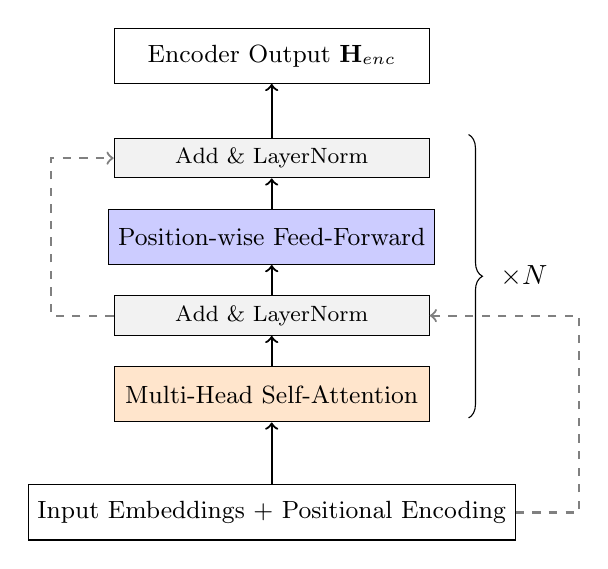
\begin{tikzpicture}[
        block/.style={rectangle, draw, minimum width=4cm, minimum height=0.7cm, align=center, font=\small},
        attn/.style={rectangle, draw, fill=orange!20, minimum width=4cm, minimum height=0.7cm, align=center, font=\small},
        ffn/.style={rectangle, draw, fill=blue!20, minimum width=4cm, minimum height=0.7cm, align=center, font=\small},
        add/.style={rectangle, draw, fill=gray!10, minimum width=4cm, minimum height=0.5cm, align=center, font=\footnotesize},
        arrow/.style={->, thick}
    ]
        % Input
        \node[block] (input) at (0, 0) {Input Embeddings + Positional Encoding};

        % Encoder block
        \node[attn] (attn) at (0, 1.5) {Multi-Head Self-Attention};
        \node[add] (add1) at (0, 2.5) {Add \& LayerNorm};
        \node[ffn] (ffn) at (0, 3.5) {Position-wise Feed-Forward};
        \node[add] (add2) at (0, 4.5) {Add \& LayerNorm};

        % Arrows
        \draw[arrow] (input) -- (attn);
        \draw[arrow] (attn) -- (add1);
        \draw[arrow] (add1) -- (ffn);
        \draw[arrow] (ffn) -- (add2);

        % Residual connections
        \draw[arrow, dashed, gray] (input.east) -- ++(0.8, 0) |- (add1.east);
        \draw[arrow, dashed, gray] (add1.west) -- ++(-0.8, 0) |- (add2.west);

        % N times
        \draw[decorate, decoration={brace, amplitude=5pt, mirror}] (2.5, 1.2) -- (2.5, 4.8) node[midway, right=8pt] {$\times N$};

        % Output
        \node[block] (output) at (0, 5.8) {Encoder Output $\mathbf{H}_{\text{enc}}$};
        \draw[arrow] (add2) -- (output);
    \end{tikzpicture}
    \caption{Transformer encoder block. Each layer contains multi-head self-attention followed by a position-wise feed-forward network, with residual connections and layer normalisation around each sub-layer. The encoder consists of $N$ identical stacked blocks.}
    \label{fig:transformer-encoder}
\end{figure}

\subsection{Transformer Decoder}

\begin{rigour}[Transformer Decoder Block]
Each decoder block has three sub-layers:

\textbf{1. Masked Multi-Head Self-Attention:}
\[
\mathbf{Z}_1 = \text{MaskedMultiHead}(\mathbf{Y}, \mathbf{Y}, \mathbf{Y})
\]
\textbf{Masking prevents attending to future positions:} When generating token $t$, the decoder can only attend to positions $\leq t$.

\textbf{2. Multi-Head Cross-Attention:}
\[
\mathbf{Z}_2 = \text{MultiHead}(\mathbf{Z}_1, \mathbf{H}_{\text{enc}}, \mathbf{H}_{\text{enc}})
\]
\begin{itemize}
    \item Queries: from decoder ($\mathbf{Z}_1$)
    \item Keys and values: from encoder output ($\mathbf{H}_{\text{enc}}$)
\end{itemize}
This allows the decoder to attend to the input sequence.

\textbf{3. Position-wise Feed-Forward Network:}

Same structure as encoder FFN.

\textbf{Full decoder block:}
\begin{align*}
\mathbf{Z}_1 &= \text{LayerNorm}(\mathbf{Y} + \text{MaskedMultiHead}(\mathbf{Y}, \mathbf{Y}, \mathbf{Y})) \\
\mathbf{Z}_2 &= \text{LayerNorm}(\mathbf{Z}_1 + \text{MultiHead}(\mathbf{Z}_1, \mathbf{H}_{\text{enc}}, \mathbf{H}_{\text{enc}})) \\
\mathbf{Z}_3 &= \text{LayerNorm}(\mathbf{Z}_2 + \text{FFN}(\mathbf{Z}_2))
\end{align*}
\end{rigour}

\begin{redbox}
\textbf{Why Masked Attention?}

During training, we have the full target sequence. Without masking, position $t$ could ``cheat'' by looking at positions $t+1, t+2, \ldots$

\textbf{Causal masking} prevents this:
\[
\text{Mask}_{ij} = \begin{cases} 0 & \text{if } j \leq i \\ -\infty & \text{if } j > i \end{cases}
\]

Adding this mask before softmax ensures $\alpha_{ij} = 0$ for $j > i$.

During inference, masking is naturally satisfied since future tokens do not exist yet.
\end{redbox}

\subsection{Transformer Variants}

\begin{quickref}[Transformer Architecture Types]
\textbf{1. Encoder-Decoder (Original Transformer, T5, BART):}
\begin{itemize}
    \item Full encoder processes input sequence
    \item Full decoder generates output autoregressively
    \item Best for: translation, summarisation, sequence-to-sequence tasks
\end{itemize}

\textbf{2. Encoder-Only (BERT, RoBERTa):}
\begin{itemize}
    \item Only encoder stack
    \item Bidirectional attention (no masking)
    \item Output: contextualised representations for each input token
    \item Best for: classification, NER, question answering, embedding
\end{itemize}

\textbf{3. Decoder-Only (GPT, LLaMA, Claude):}
\begin{itemize}
    \item Only decoder stack (with causal masking)
    \item Unidirectional: each token attends only to previous tokens
    \item Best for: text generation, language modelling, completion
\end{itemize}
\end{quickref}

%==============================================================================
\section{BERT: Encoder-Only Transformer}
\label{sec:bert}
%==============================================================================

BERT (Bidirectional Encoder Representations from Transformers) demonstrated the power of pretraining transformer encoders on large text corpora.

\begin{rigour}[BERT Architecture and Pretraining]
\textbf{Architecture:}
\begin{itemize}
    \item Encoder-only transformer (no decoder)
    \item Bidirectional: each token attends to all other tokens
    \item BERT-Base: 12 layers, 768 hidden, 12 heads, 110M parameters
    \item BERT-Large: 24 layers, 1024 hidden, 16 heads, 340M parameters
\end{itemize}

\textbf{Pretraining Task 1: Masked Language Modelling (MLM)}
\begin{enumerate}
    \item Randomly mask 15\% of input tokens
    \item Of masked positions: 80\% replaced with \texttt{[MASK]}, 10\% random token, 10\% unchanged
    \item Objective: predict original tokens at masked positions
\end{enumerate}

\textbf{Example:}
\begin{itemize}
    \item Input: ``The cat [MASK] on the mat''
    \item Target: predict ``sat'' at masked position
\end{itemize}

\textbf{Pretraining Task 2: Next Sentence Prediction (NSP)}
\begin{itemize}
    \item Given two sentences, predict whether B follows A in the original text
    \item 50\% positive pairs (consecutive), 50\% negative pairs (random)
\end{itemize}

\textbf{Key insight:} MLM is \textbf{self-supervised}-no manual labelling required. The training signal comes from the text itself.
\end{rigour}

\begin{quickref}[BERT Variants]
\begin{itemize}
    \item \textbf{RoBERTa} (Robustly Optimised BERT): Trained longer on more data, removes NSP task
    \item \textbf{ALBERT} (A Lite BERT): Parameter sharing across layers for efficiency
    \item \textbf{SpanBERT}: Masks contiguous spans rather than random tokens
    \item \textbf{DistilBERT}: Smaller model via knowledge distillation (40\% smaller, 60\% faster)
    \item \textbf{Domain-specific BERTs}: ClimateBERT, BioBERT, LegalBERT-pretrained on domain corpora
\end{itemize}
\end{quickref}

\begin{quickref}[Using BERT for Downstream Tasks]
\textbf{Fine-tuning approach:}
\begin{enumerate}
    \item Take pretrained BERT model
    \item Add task-specific head (e.g., classification layer)
    \item Fine-tune entire model on task-specific labelled data
\end{enumerate}

\textbf{Common tasks:}
\begin{itemize}
    \item \textbf{Classification:} Use \texttt{[CLS]} token representation $\rightarrow$ softmax classifier
    \item \textbf{Named Entity Recognition:} Use each token's representation $\rightarrow$ token-level classification
    \item \textbf{Question Answering:} Predict start/end positions of answer span
\end{itemize}

\textbf{Transfer learning benefit:} Pretrained representations capture general language understanding, requiring less task-specific data for good performance.
\end{quickref}

%==============================================================================
\section{Vision Transformer (ViT)}
\label{sec:vit}
%==============================================================================

The Vision Transformer adapts the transformer architecture from NLP to computer vision, treating images as sequences of patches.

\begin{rigour}[Vision Transformer Architecture]
\textbf{Key insight:} An image can be treated as a sequence of patches, analogous to a sequence of word tokens.

\textbf{Process:}
\begin{enumerate}
    \item \textbf{Patch extraction:} Divide image into fixed-size patches (e.g., $16 \times 16$ pixels)

    For image size $H \times W$ with patch size $P \times P$:
    \[
    N = \frac{H \times W}{P^2} \text{ patches}
    \]

    \item \textbf{Linear projection:} Flatten each patch to a vector and project to embedding dimension $D$:
    \[
    \mathbf{z}_i = \mathbf{x}_{\text{patch}_i} \mathbf{E} + \mathbf{e}_{\text{pos}_i}
    \]
    where $\mathbf{E} \in \mathbb{R}^{P^2 \cdot C \times D}$ is the projection matrix and $\mathbf{e}_{\text{pos}_i}$ is the position embedding.

    \item \textbf{Class token:} Prepend a learnable \texttt{[CLS]} token embedding $\mathbf{z}_0$

    \item \textbf{Transformer encoder:} Process patch embeddings through $L$ transformer encoder layers

    \item \textbf{Classification head:} Use the \texttt{[CLS]} token output for classification:
    \[
    \hat{y} = \text{MLP}(\mathbf{z}_0^{(L)})
    \]
\end{enumerate}

\textbf{Dimensions:}
\begin{itemize}
    \item Input image: $224 \times 224 \times 3$ (RGB)
    \item Patch size: $16 \times 16$
    \item Number of patches: $14 \times 14 = 196$
    \item Sequence length: $196 + 1 = 197$ (including \texttt{[CLS]})
\end{itemize}
\end{rigour}

\begin{figure}[H]
    \centering
    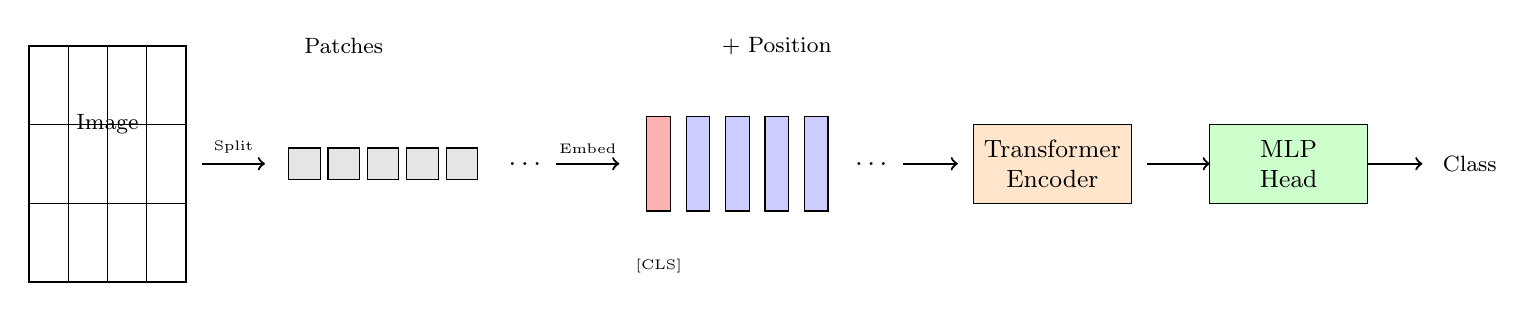
\begin{tikzpicture}[
        patch/.style={rectangle, draw, minimum size=0.4cm, fill=gray!20},
        emb/.style={rectangle, draw, fill=blue!20, minimum width=0.3cm, minimum height=1.2cm},
        cls/.style={rectangle, draw, fill=red!30, minimum width=0.3cm, minimum height=1.2cm},
        block/.style={rectangle, draw, minimum width=2cm, minimum height=1cm, align=center, font=\small},
        arrow/.style={->, thick}
    ]
        % Original image
        \node at (-4.5, 1.5) {\footnotesize Image};
        \draw[thick] (-5.5, -0.5) rectangle (-3.5, 2.5);
        % Grid of patches
        \foreach \x in {0, 1, 2, 3} {
            \foreach \y in {0, 1, 2} {
                \draw (-5.5+\x*0.5, -0.5+\y*1.0) rectangle (-5.0+\x*0.5, 0.5+\y*1.0);
            }
        }

        % Arrow
        \draw[arrow] (-3.3, 1) -- (-2.5, 1) node[midway, above] {\tiny Split};

        % Patches flattened
        \node at (-1.5, 2.5) {\footnotesize Patches};
        \foreach \i in {0, 1, 2, 3, 4} {
            \node[patch] at (-2+\i*0.5, 1) {};
        }
        \node at (0.8, 1) {$\ldots$};

        % Arrow
        \draw[arrow] (1.2, 1) -- (2, 1) node[midway, above] {\tiny Embed};

        % Embeddings with class token
        \node at (4, 2.5) {\footnotesize + Position};
        \node[cls] (c) at (2.5, 1) {};
        \node at (2.5, -0.3) {\tiny [CLS]};
        \foreach \i in {1, 2, 3, 4} {
            \node[emb] at (2.5+\i*0.5, 1) {};
        }
        \node at (5.2, 1) {$\ldots$};

        % Transformer
        \draw[arrow] (5.6, 1) -- (6.3, 1);
        \node[block, fill=orange!20] (trans) at (7.5, 1) {Transformer\\Encoder};

        % Classification head
        \draw[arrow] (8.7, 1) -- (9.5, 1);
        \node[block, fill=green!20] (mlp) at (10.5, 1) {MLP\\Head};

        % Output
        \draw[arrow] (11.5, 1) -- (12.2, 1);
        \node at (12.8, 1) {\footnotesize Class};
    \end{tikzpicture}
    \caption{Vision Transformer (ViT) architecture. An image is divided into fixed-size patches, which are flattened and linearly projected to embeddings. A learnable \texttt{[CLS]} token is prepended, positional embeddings are added, and the sequence is processed by a standard Transformer encoder. The \texttt{[CLS]} token output is used for classification.}
    \label{fig:vit-architecture}
\end{figure}

\begin{quickref}[ViT Performance Characteristics]
\textbf{Comparison with CNNs:}
\begin{itemize}
    \item ViT \textbf{outperforms ResNets} of comparable computational budget when trained on sufficient data
    \item ViT does \textbf{not saturate} in performance-continues improving with more compute/data
    \item CNNs have useful \textbf{inductive biases} (locality, translation equivariance) that help with limited data
\end{itemize}

\textbf{Data requirements:}
\begin{itemize}
    \item ViT trained on ImageNet-1k (1.3M images): underperforms CNNs
    \item ViT trained on ImageNet-21k (14M images): matches CNNs
    \item ViT trained on JFT-300M (300M images): significantly outperforms CNNs
\end{itemize}

\textbf{Key insight:} Transformers lack the built-in assumptions of CNNs, requiring more data to learn equivalent representations, but can ultimately learn more powerful representations given sufficient data.
\end{quickref}

\begin{redbox}
\textbf{ViT Data Requirements}

Vision Transformers require \textbf{very large datasets} to outperform CNNs significantly.

\textbf{Why?}
\begin{itemize}
    \item CNNs have \textbf{inductive biases}: locality (nearby pixels are related) and translation equivariance (patterns are position-independent)
    \item Transformers must \textbf{learn these patterns from data}
    \item With limited data, CNNs' built-in assumptions help generalisation
    \item With abundant data, transformers' flexibility becomes advantageous
\end{itemize}

\textbf{Practical implication:} For most vision tasks with limited labelled data, CNNs or hybrid architectures may be more appropriate. ViT shines in large-scale pretraining settings.
\end{redbox}

%==============================================================================
\section{Computational Considerations}
\label{sec:computational}
%==============================================================================

Understanding the computational properties of transformers is essential for practical deployment.

\begin{rigour}[Transformer Complexity Analysis]
For sequence length $n$ and model dimension $d$:

\textbf{Self-attention:}
\begin{itemize}
    \item Attention scores: $\mathbf{Q}\mathbf{K}^\top$ requires $O(n^2 \cdot d)$ operations
    \item Memory for attention matrix: $O(n^2)$
    \item Weighted sum: $O(n^2 \cdot d)$
\end{itemize}

\textbf{Feed-forward network:}
\begin{itemize}
    \item Typically expands to $4d$ hidden units
    \item Two linear layers: $O(n \cdot d \cdot 4d) = O(n \cdot d^2)$
\end{itemize}

\textbf{Total per layer:} $O(n^2 \cdot d + n \cdot d^2)$

\textbf{Comparison:}
\begin{center}
\begin{tabular}{lcc}
\textbf{Operation} & \textbf{Complexity} & \textbf{Sequential Ops} \\
\hline
Self-attention & $O(n^2 \cdot d)$ & $O(1)$ \\
RNN & $O(n \cdot d^2)$ & $O(n)$ \\
CNN (kernel $k$) & $O(k \cdot n \cdot d^2)$ & $O(\log_k n)$ \\
\end{tabular}
\end{center}

Self-attention has $O(1)$ sequential operations (fully parallel) but quadratic in sequence length.
\end{rigour}

\begin{quickref}[Practical Implications]
\textbf{When sequence length dominates ($n > d$):}
\begin{itemize}
    \item Self-attention becomes the bottleneck
    \item Consider efficient attention variants (sparse, linear)
\end{itemize}

\textbf{When model dimension dominates ($d > n$):}
\begin{itemize}
    \item FFN layers become the bottleneck
    \item Standard transformers work well
\end{itemize}

\textbf{Typical regime:} $d = 768$ or $d = 1024$, $n = 512$ or $n = 2048$. Both terms contribute significantly.

\textbf{Modern scaling:} Large language models use $n$ up to 100,000+, requiring specialised attention implementations (Flash Attention, sparse patterns).
\end{quickref}

%==============================================================================
\section{Summary: The Attention Revolution}
\label{sec:summary}
%==============================================================================

\begin{quickref}[Week 8 Summary]
\textbf{Encoder-Decoder Architecture:}
\begin{itemize}
    \item Framework for seq2seq: compress input to fixed context, decode to variable output
    \item Vanilla RNN version suffers from information bottleneck for long sequences
    \item BLEU metric evaluates translation quality via n-gram precision
\end{itemize}

\textbf{Attention Mechanism:}
\begin{itemize}
    \item Query-Key-Value framework enables selective focus
    \item Additive attention: for different-dimension Q/K
    \item Scaled dot-product attention: efficient, used in transformers
    \item Bahdanau attention: dynamic context for each decoder step
    \item Multi-head attention: parallel attention with different projections
    \item Self-attention: sequence attends to itself; enables parallel computation and direct long-range connections
\end{itemize}

\textbf{Transformer:}
\begin{itemize}
    \item Built entirely on attention-no recurrence or convolution
    \item Positional encoding injects sequence order information
    \item Encoder: self-attention + FFN with residuals and layer norm
    \item Decoder: masked self-attention + cross-attention + FFN
    \item Variants: encoder-only (BERT), decoder-only (GPT), encoder-decoder (T5)
\end{itemize}

\textbf{Pretrained Models:}
\begin{itemize}
    \item BERT: masked language modelling enables bidirectional pretraining
    \item ViT: treats images as patch sequences; powerful but data-hungry
\end{itemize}

\textbf{Key Equations:}
\begin{align*}
    \text{Scaled dot-product:} \quad & a(\mathbf{q}, \mathbf{k}) = \frac{\mathbf{q}^\top \mathbf{k}}{\sqrt{d}} \\
    \text{Self-attention:} \quad & \mathbf{y}_i = \sum_{j=1}^{n} \text{softmax}\left(\frac{\mathbf{x}_i^\top \mathbf{x}_j}{\sqrt{d}}\right) \mathbf{x}_j \\
    \text{Bahdanau context:} \quad & \mathbf{c}_{t'} = \sum_{t=1}^{T} \alpha(\mathbf{s}_{t'-1}, \mathbf{h}_t) \mathbf{h}_t
\end{align*}

\textbf{Caveats:}
\begin{itemize}
    \item Self-attention has $O(n^2)$ complexity-problematic for very long sequences
    \item Teacher forcing creates train-test mismatch
    \item ViT requires massive datasets to outperform CNNs
\end{itemize}
\end{quickref}

%==============================================================================
\section{Connections to Other Topics}
\label{sec:connections}
%==============================================================================

\begin{quickref}[Cross-References and Connections]
\textbf{Building on previous chapters:}
\begin{itemize}
    \item \textbf{Chapter~\ref{ch:week6} (RNNs and LSTMs):} Encoder-decoder models originally used RNNs; understanding their limitations (vanishing gradients, sequential processing) motivates attention
    \item \textbf{Chapter~\ref{ch:week7} (Word Embeddings):} Token embeddings (Word2Vec, GloVe) provide the input representations that Transformers process; BERT generates contextual embeddings as discussed there
\end{itemize}

\textbf{Key architectural concepts from earlier chapters:}
\begin{itemize}
    \item \textbf{Residual connections} (Chapter~\ref{ch:week5}): Critical for training deep Transformers, enabling gradient flow through many layers
    \item \textbf{Regularisation techniques} (Chapter~\ref{ch:week7}): Dropout is applied within Transformer layers to prevent overfitting
    \item \textbf{Layer normalisation}: Stabilises training similarly to batch normalisation discussed in CNN chapters
\end{itemize}

\textbf{Forward connections:}
\begin{itemize}
    \item \textbf{Chapter~\ref{ch:week9} (LLMs in Practice):} Will explore how large Transformer models are deployed, including prompting strategies and fine-tuning
    \item \textbf{Transfer learning}: BERT exemplifies the pre-train then fine-tune paradigm that has become dominant in modern deep learning
\end{itemize}

\textbf{Broader context:}
\begin{itemize}
    \item The attention mechanism has unified architectures across modalities: text (GPT, BERT), images (ViT), audio (Whisper), and multimodal (CLIP, Flamingo)
    \item Understanding Transformers is essential for working with any modern foundation model
\end{itemize}
\end{quickref}

%==============================================================================
% References
%==============================================================================

\begin{rigour}[Key References]
\begin{itemize}
    \item Zhang et al., ``Dive into Deep Learning,'' Chapters 10--11
    \item Vaswani et al. (2017), ``Attention Is All You Need''-introduced the Transformer
    \item Bahdanau et al. (2015), ``Neural Machine Translation by Jointly Learning to Align and Translate''-Bahdanau attention
    \item Devlin et al. (2019), ``BERT: Pre-training of Deep Bidirectional Transformers for Language Understanding''
    \item Dosovitskiy et al. (2021), ``An Image is Worth 16x16 Words: Transformers for Image Recognition at Scale''-Vision Transformer
    \item Brown et al. (1990), ``A Statistical Approach to Machine Translation''-word alignment in MT
\end{itemize}
\end{rigour}
